\let\negmedspace\undefined
\let\negthickspace\undefined
\documentclass[journal]{IEEEtran}
\usepackage[a5paper, margin=10mm, onecolumn]{geometry}
\usepackage{tfrupee} 

\setlength{\headheight}{1cm} 
\setlength{\headsep}{0mm}  
\usepackage{gvv-book}
\usepackage{gvv}
\usepackage{cite}
\usepackage{amsmath,amssymb,amsfonts,amsthm}
\usepackage{algorithmic}
\usepackage{graphicx}
\usepackage{textcomp}
\usepackage{xcolor}
\usepackage{txfonts}
\usepackage{listings}
\usepackage{enumitem}
\usepackage{mathtools}
\usepackage{gensymb}
\usepackage{comment}
\usepackage[breaklinks=true]{hyperref}
\usepackage{tkz-euclide} 
\usepackage{listings}
% \usepackage{gvv}                                        
\def\inputGnumericTable{}                                 
\usepackage[latin1]{inputenc}                                
\usepackage{color}                                            
\usepackage{array}                                            
\usepackage{longtable}                                       
\usepackage{calc}                                             
\usepackage{multirow}                                         
\usepackage{hhline}                                           
\usepackage{ifthen}                                           
\usepackage{lscape}
\usepackage{tikz}
\usetikzlibrary{patterns}
\begin{document}

\bibliographystyle{IEEEtran}
\vspace{3cm}


\title{GATE 2009 ME }
\author{ee25btech11029- Jnanesh Sathisha Karmar}
\maketitle
% \maketitle
% \newpage
% \bigskip
{\let\newpage\relax\maketitle}

\renewcommand{\thefigure}{\theenumi}
\renewcommand{\thetable}{\theenumi}
\setlength{\intextsep}{10pt} % Space between text and floats
\begin{enumerate}[leftmargin=0pt]


    \item The product of eigenvalues of the matrix $P = \myvec{2 & 0 \\ 4 & -3}$ is
    
    \hfill{\brak{\text{GATE ME 2017}}}

    \begin{enumerate}
        \begin{multicols}{4}
            \item $-6$
            \item $2$
            \item $6$
            \item $-2$
        \end{multicols}
    \end{enumerate}
    
    \item The value of $\displaystyle\lim_{x \to 0} \frac{x^3 - \sin x}{x}$ is

    \hfill{\brak{\text{GATE ME 2017}}}

    \begin{enumerate}
        \begin{multicols}{4}
            \item $0$
            \item $3$
            \item $-1$
            \item $-2$
        \end{multicols}
    \end{enumerate}

    \item Consider the following partial differential equation for $u(x, y)$ with the constant $c > 1$:
    \begin{align*}
        \frac{\partial u}{\partial y} + c \frac{\partial u}{\partial x} = 0
    \end{align*}
    Solution of this equation is

    \hfill{\brak{\text{GATE ME 2017}}}

    \begin{enumerate}
        \begin{multicols}{4}
            \item $u(x, y) = f(x + cy)$
            \item $u(x, y) = f(x - cy)$
            \item $u(x, y) = f(cx + y)$
            \item $u(x, y) = f(cx - y)$
        \end{multicols}
    \end{enumerate}
    
    \item The differential equation $\frac{d^2 y}{dx^2} + 16y = 0$ for $y(x)$ with the two boundary conditions $\frac{dy}{dx}\bigg|_{x=0} = 1$ and $\frac{dy}{dx}\bigg|_{x=\frac{\pi}{2}} = -1$ has

    \hfill{\brak{\text{GATE ME 2017}}}

    \begin{enumerate}
        \begin{multicols}{4}
            \item no solution
            \item exactly two solutions
            \item exactly one solution
            \item infinitely many solutions
        \end{multicols}
    \end{enumerate}

    \item A six-face fair dice is rolled a large number of times. The mean value of the outcomes is
        $\underline{\hspace{2cm}}$

    \hfill{\brak{\text{GATE ME 2017}}}

    \item For steady flow of a viscous incompressible fluid through a circular pipe of constant diameter, the average velocity in the fully developed region is constant. Which one of the following statements about the average velocity in the developing region is TRUE?

    \hfill{\brak{\text{GATE ME 2017}}}

    \begin{enumerate}
        \begin{multicols}{4}
            \item It increases until the flow is fully developed.
            \item It is constant and is equal to the average velocity in the fully developed region.
            \item It decreases until the flow is fully developed.
            \item It is constant but is always lower than the average velocity in the fully developed region.
        \end{multicols}
    \end{enumerate}

    \item Consider the two-dimensional velocity field given by $\vec{V} = (5 + a_1 x + b_1 y)\hat{i} + (4 + a_2 x + b_2 y)\hat{j}$, where $a_1, b_1, a_2, b_2$ are constants. Which one of the following conditions needs to be satisfied for the flow to be incompressible?

    \hfill{\brak{\text{GATE ME 2017}}}

    \begin{enumerate}
        \begin{multicols}{4}
            \item $a_1 + b_1 = 0$
            \item $a_1 + b_2 = 0$
            \item $a_2 + b_2 = 0$
            \item $a_2 + b_1 = 0$
        \end{multicols}
    \end{enumerate}

    \item Water (density $= 1000\text{ kg/m}^3$) at ambient temperature flows through a horizontal pipe of uniform cross section at the rate of $1\text{ kg/s}$. If the pressure drop across the pipe is $100\text{ kPa}$, the minimum power required to pump the water across the pipe, in watts, is
    $\underline{\hspace{2cm}}$

    \hfill{\brak{\text{GATE ME 2017}}}

    \item Which one of the following is NOT a rotating machine?

    \hfill{\brak{\text{GATE ME 2017}}}

    \begin{enumerate}
        \begin{multicols}{4}
            \item Centrifugal pump
            \item Gear pump
            \item Jet pump
            \item Vane pump
        \end{multicols}
    \end{enumerate}

    \item Saturated steam at $100\degree$C condenses on the outside of a tube. Cold fluid enters the tube at $20\degree$C and exits at $50\degree$C. The value of the Log Mean Temperature Difference (LMTD) is
        $\underline{\hspace{2cm}} \degree$C.

    \hfill{\brak{\text{GATE ME 2017}}}

    \item The molar specific heat at constant volume of an ideal gas is equal to $2.5$ times the universal gas constant $(8.314\,\text{J}/\text{mol}\cdot\text{K})$. When the temperature increases by $100$K, the change in molar specific enthalpy is 
        $\underline{\hspace{2cm}}$J/mol.

    \hfill{\brak{\text{GATE ME 2017}}}

    \item A heat pump absorbs $10$kW of heat from outside environment at $250$K while absorbing $15$kW of work. It delivers the heat to a room that must be kept warm at $300$K. The Coefficient of Performance (COP) of the heat pump is
        $\underline{\hspace{2cm}}$

    \hfill{\brak{\text{GATE ME 2017}}}

    \item The Poisson's ratio for a perfectly incompressible linear elastic material is 

    \hfill{\brak{\text{GATE ME 2017}}}

    \begin{enumerate}
        \begin{multicols}{4}
            \item $1$
            \item $0.5$
            \item $0$
            \item infinity
        \end{multicols}
    \end{enumerate}

    \item A particle of unit mass is moving on a plane. Its trajectory, in polar coordinates, is given by $r(t) = t^2,\,\theta(t) = t$ where $t$ is time. The kinetic energy of the particle at time $t = 2$ is

    \hfill{\brak{\text{GATE ME 2017}}}

    \begin{enumerate}
        \begin{multicols}{4}
            \item $4$
            \item $12$
            \item $16$
            \item $24$
        \end{multicols}
    \end{enumerate}

    \item A motor driving a solid circular steel shaft transmits $40$kW of power at $500$rpm. If the diameter of the shaft is $40$mm, the maximum shear stress in the shaft is
    $\underline{\hspace{2cm}}$MPa.

    \hfill{\brak{\text{GATE ME 2017}}}

    \item Consider a beam with circular cross-section of diameter $d$. The ratio of the second moment of area about the neutral axis to the section modulus of the area is

    \hfill{\brak{\text{GATE ME 2017}}}

    \begin{enumerate}
        \begin{multicols}{4}
            \item $\displaystyle\frac{2}{\pi d}$
            \item $2$
            \item $d$
            \item $\displaystyle\frac{d}{\pi}$
        \end{multicols}
    \end{enumerate}

    \item The following figure shows the velocity-time plot for a particle traveling along a straight line. The distance covered by the particle from $t = 0$ to $t = 5$ s is
    $\underline{\hspace{2cm}}$m.
    \begin{figure}[h]
\centering
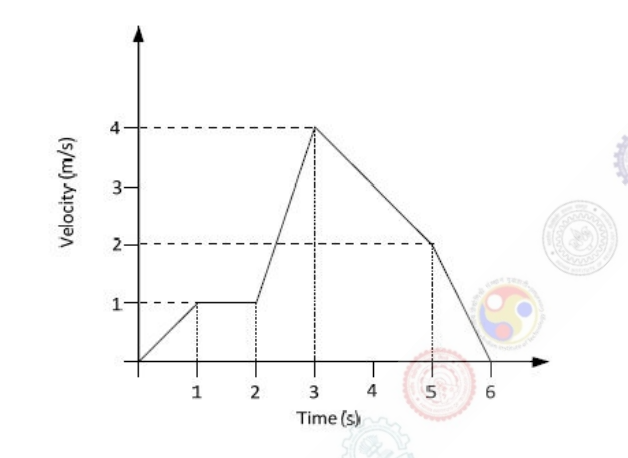
\includegraphics[width=0.5\columnwidth]{Figs/image (22).png}
\caption*{}
\label{fig:17}
\end{figure}

    \hfill{\brak{\text{GATE ME 2017}}}


    \item The damping ratio for a viscously damped spring mass system, governed by the relationship
    \[
        m \frac{d^2 x}{dt^2} + c \frac{dx}{dt} + k x = F(t)
    \]
    is given by

    \hfill{\brak{\text{GATE ME 2017}}}
    
    \begin{enumerate}
        \begin{multicols}{4}
            \item $\sqrt{\frac{C}{mk}}$
            \item $\frac{C}{2\sqrt{km}}$
            \item $\frac{C}{\sqrt{km}}$
            \item $\sqrt{\frac{C}{2mk}}$
        \end{multicols}
    \end{enumerate}
    
    \item Consider the schematic of a riveted lap joint subjected to tensile load $F$, as shown below. Let $d$ be the diameter of the rivets, and $S$ be the maximum permissible tensile stress in the plates. What should be the minimum value for the thickness of the plates to guard against tensile failure of the plates? Assume the plates to be identical.
    \begin{figure}[h]
\centering
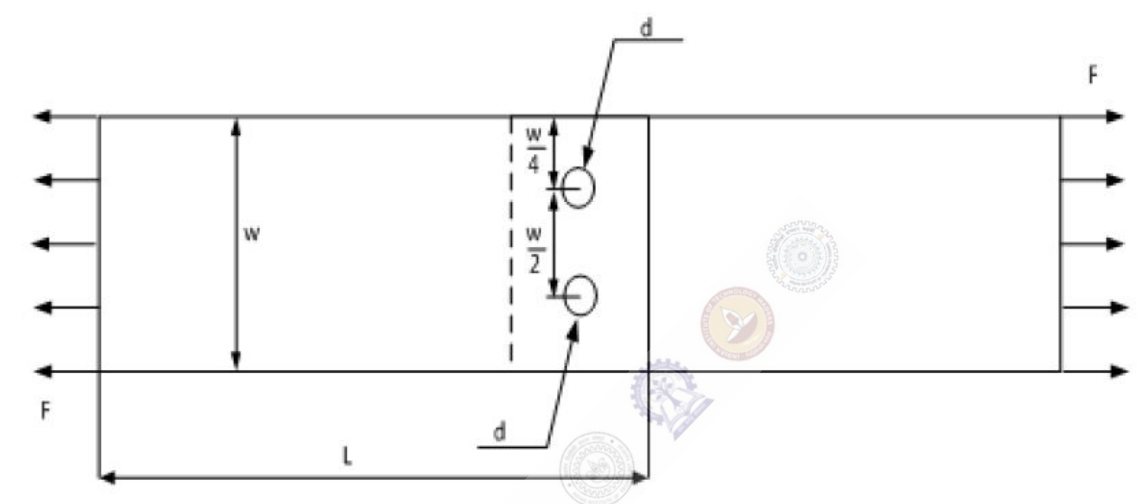
\includegraphics[width=0.5\columnwidth]{Figs/image (23).png}
\caption*{}
\label{fig:19}
\end{figure}

    \hfill{\brak{\text{GATE ME 2017}}}

    \begin{enumerate}
        \begin{multicols}{4}
            \item $sp(W-2d)$
            \item $SW$
            \item $Sf(W-d)$
            \item $SFW$
        \end{multicols}
    \end{enumerate}

    \item Cylindrical pins of diameter $15 \pm 0.020$mm are being produced on a machine. Statistical quality control tests show a mean of $14.995$mm and standard deviation of $0.004$mm. The process capability index $\text{Cp}$ is

    \hfill{\brak{\text{GATE ME 2017}}}

    \begin{enumerate}
        \begin{multicols}{4}
            \item $0.833$
            \item $1.667$
            \item $3.333$
            \item $3.750$
        \end{multicols}
    \end{enumerate}

    \item In a metal forming operation when the material has just started yielding, the principal stresses are $\sigma_1 = +180$ MPa, $\sigma_2 = -100$ MPa, $\sigma_3 = 0$. Following von Mises' criterion, the yield stress is $\underline{\hspace{2cm}}$ MPa.
    \hfill{\brak{\text{GATE ME 2017}}}

    \item Match the processes with their characteristics.
\begin{table}[h]
    \centering
    \begin{center}
\begin{tabular}{ll}
    \textbf{Group I} & \textbf{Group II} \\
    P. Ferrite & 1. Hexagonal Close Packed (HCP) \\
    Q. Austenite & 2. Body Centered Cubic (BCC) \\
    R. Martensite & 3. Body Centered Tetragonal (BCT) \\
    & 4. Face Centered Cubic (FCC)
\end{tabular}
\end{center}
\end{table}
\hfill{\brak{\text{GATE ME 2017}}}
    \begin{enumerate}
        \begin{multicols}{4}
            \item P-2, Q-3, R-1, S-4
            \item P-3, Q-2, R-1, S-4
            \item P-3, Q-2, R-4, S-1
            \item P-2, Q-4, R-3, S-1
        \end{multicols}
    \end{enumerate}

    \item In an arc welding process, welding speed is doubled. Assuming all other process parameters to be constant, the cross sectional area of the weld bead will
    \hfill{\brak{\text{GATE ME 2017}}}
    \begin{enumerate}
        \begin{multicols}{4}
            \item increase by $25\%$
            \item increase by $50\%$
            \item reduce by $25\%$
            \item reduce by $50\%$
        \end{multicols}
    \end{enumerate}

    \item Metric thread of $0.8$ mm pitch is to be cut on a lathe. Pitch of the lead screw is $1.5$ mm. If the spindle rotates at $1500$ rpm, the speed of rotation of the lead screw (rpm) will be $\underline{\hspace{2cm}}$
    \hfill{\brak{\text{GATE ME 2017}}}

    \item In the engineering stress-strain curve for mild steel, the Ultimate Tensile Strength (UTS) refers to
    \hfill{\brak{\text{GATE ME 2017}}}
    \begin{enumerate}
        \begin{multicols}{4}
            \item Yield stress
            \item Proportional limit
            \item Maximum stress
            \item Fracture stress
        \end{multicols}
    \end{enumerate}

    \item Consider the matrix P = \myvec{1 & 1 & \sqrt{2} \\ 0 & -1 & \sqrt{2} \\ 0 & 1 & 1 }. Which one of the following statements about $P$ is INCORRECT?
    \hfill{\brak{\text{GATE ME 2017}}}
    \begin{enumerate}
        \begin{multicols}{4}
            \item Determinant of $P$ is equal to $1$
            \item $P$ is orthogonal
            \item Inverse of $P$ is equal to its transpose
            \item All eigenvalues of $P$ are real numbers
        \end{multicols}
    \end{enumerate}

    \item For the vector $\mathbf{V} = 2yz\,\mathbf{i} + 3xz\,\mathbf{j} + 4xy\,\mathbf{k}$, the value of $\mathbf{V} \cdot (\mathbf{V} \times \mathbf{V})$ is $\underline{\hspace{2cm}}$
    \hfill{\brak{\text{GATE ME 2017}}}

    \item A parametric curve defined by $x = \cos \frac{\pi u}{2},\,y = 2\sin\frac{\pi u}{2}$ in the range $0 \leq u \leq 1$ is rotated about the X-axis by $360^\circ$. Area of the surface generated is
    \hfill{\brak{\text{GATE ME 2017}}}
    \begin{enumerate}
        \begin{multicols}{4}
            \item $\frac{\pi}{2}$
            \item $\pi$
            \item $2\pi$
            \item $4\pi$
        \end{multicols}
    \end{enumerate}

    \item $P(0,3),$ $Q(0.5,4),$ and $R(1,5)$ are three points on the curve defined by $f(x)$. Numerical integration is carried out using both Trapezoidal rule and Simpson's rule within limits $x = 0$ and $x = 1$ for the curve. The difference between the two results will be
    \hfill{\brak{\text{GATE ME 2017}}}
    \begin{enumerate}
        \begin{multicols}{4}
            \item $0$
            \item $0.25$
            \item $0.5$
            \item $1$
        \end{multicols}
    \end{enumerate}

    \item The velocity profile inside the boundary layer for flow over a flat plate is given as $u = U_\infty \sin \frac{\pi y}{\delta}$ where $U$ is the free stream velocity and $\delta$ is the local boundary layer thickness. If $\delta^*$ is the local displacement thickness, the value of $\frac{\delta^*}{\delta}$ is
    \hfill{\brak{\text{GATE ME 2017}}}
    \begin{enumerate}
        \begin{multicols}{4}
            \item $\frac{\pi}{2}$
            \item $1$
            \item $\frac{2}{\pi}$
            \item $\frac{1+\pi}{0}$
        \end{multicols}
    \end{enumerate}

    \item Consider steady flow of an incompressible fluid through two long and straight pipes of diameters $d_1$ and $d_2$ arranged in series. Both pipes are of equal length and the flow is turbulent in both pipes. The friction factor for turbulent flow though pipes is of the form $f = K (\text{Re})^{-n}$, where $K$ and $n$ are known positive constants and Re is Reynolds number. Neglecting minor losses, the ratio of the frictional pressure drop in pipe 1 to that in pipe 2, $\frac{\Delta P_1}{\Delta P_2}$ is given by:
    \hfill{\brak{\text{GATE ME 2017}}}
    \begin{enumerate}
        \begin{multicols}{4}
            \item $\left(\frac{d_1}{d_2}\right)^{5-n}$
            \item $\left(\frac{d_2}{d_1}\right)^{5-n}$
            \item $\left(\frac{d_1}{d_2}\right)^{3-n}$
            \item $\left(\frac{d_2}{d_1}\right)^{5+n}$
        \end{multicols}
    \end{enumerate}

    \item For a steady flow, the velocity field is $\mathbf{V} = (-x^2 + 3y)\mathbf{i} + (2xy)\mathbf{j}$. The magnitude of the acceleration of a particle at $(1, -1)$ is
    \hfill{\brak{\text{GATE ME 2017}}}
    \begin{enumerate}
        \begin{multicols}{4}
            \item $2$
            \item $1$
            \item $2\sqrt{5}$
            \item $0$
        \end{multicols}
    \end{enumerate}

    \item One kg of an ideal gas (gas constant $R = 400$ J/kg$\cdot$K; specific heat at constant volume $C_v = 1000$ J/kg$\cdot$K) at $1$ bar and $300$K is contained in a sealed rigid cylinder. During an adiabatic process, $100$ kJ of work is done on the system by a stirrer. The increase in entropy of the system is $\underline{\hspace{2cm}}$ J/K.
    \hfill{\brak{\text{GATE ME 2017}}}

    \item The pressure ratio across a gas turbine (for air, specific heat at constant pressure $C_p = 1040$ J/kg$\cdot$K and ratio of specific heats $\gamma = 1.4$) is $10$. If the inlet temperature to the turbine is $1200$K and the isentropic efficiency is $0.9$, the gas temperature at turbine exit is $\underline{\hspace{2cm}}$ K.
    \hfill{\brak{\text{GATE ME 2017}}}

    \item Moist air is treated as an ideal gas mixture of water vapor and dry air (molecular weight of air = $28.84$ and molecular weight of water = $18$). At a location, the total pressure is $100$ kPa, the temperature is $30\degree$C and the relative humidity is $55\%$. Given that the saturation pressure of water at $30\degree$C is $4246$ Pa, the mass of water vapor per kg of dry air is $\underline{\hspace{2cm}}$ grams.
    \hfill{\brak{\text{GATE ME 2017}}}

    \item Air contains $79\%$ N$_2$ and $21\%$ O$_2$ on a molar basis. Methane (CH$_4$) is burned with $50\%$ excess air than required stoichiometrically. Assuming complete combustion of methane, the molar percentage of N$_2$ in the products is $\underline{\hspace{2cm}}$.
    \hfill{\brak{\text{GATE ME 2017}}}

    \item Two black surfaces, AB and BC, of lengths $5$ m and $6$ m, respectively, are oriented as shown. Both surfaces extend infinitely into the third dimension. Given that view factor $F_{12} = 0.5$, $T_1 = 800$K, $T_2 = 600$K, $T_{\text{surrounding}} = 300$K and Stefan Boltzmann constant, $\sigma = 5.67 \times 10^{-8}$ W/(m$^2$K$^4$), the heat transfer rate from Surface 2 to the surrounding environment is $\underline{\hspace{2cm}}$ kW.
    \hfill{\brak{\text{GATE ME 2017}}}
    \begin{figure}[h]
    \centering
    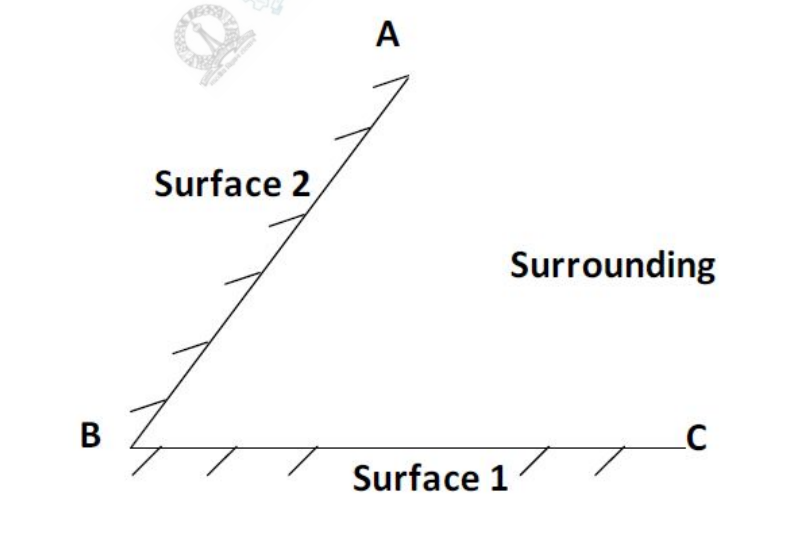
\includegraphics[width=0.5\columnwidth]{Figs/image (24).png}
    \caption*{}
    \label{fig:37}
    \end{figure}

    \item Heat is generated uniformly in a long solid cylindrical rod (diameter = $10$ mm) at the rate of $4 \times 10^7$ W/m$^3$. The thermal conductivity of the rod material is $25$ W/m$\cdot$K. Under steady state conditions, the temperature difference between the centre and the surface of the rod is $\underline{\hspace{2cm}}$ $^\circ$C.
    \hfill{\brak{\text{GATE ME 2017}}}

    \item An initially stress-free massless elastic beam of length $L$ and circular cross-section with diameter $d$ $(d \ll L)$ is held fixed between two walls as shown. The beam material has Young's modulus $E$ and coefficient of thermal expansion $\alpha$. If the beam is slowly and uniformly heated, the temperature rise required to cause the beam to buckle is proportional to
    \hfill{\brak{\text{GATE ME 2017}}}
    \begin{figure}[h]
    \centering
    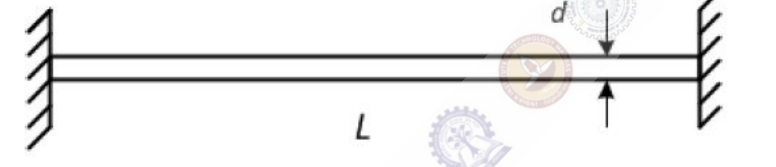
\includegraphics[width=0.5\columnwidth]{Figs/image (25).png}
    \caption*{}
    \label{fig:39}
    \end{figure}
    \newpage
    \begin{enumerate}
        \begin{multicols}{4}
            \item $d$
            \item $d^2$
            \item $d^3$
            \item $d^4$
        \end{multicols}
    \end{enumerate}

    \item A point mass of $100$ kg is dropped onto a massless elastic bar (cross-sectional area = $100$ mm$^2$, length = $1$ m, Young's modulus = $100$ GPa) from a height $H$ of $10$ mm as shown (Figure is not to scale). If $g = 10$ m/s$^2$, the maximum compression of the elastic bar is $\underline{\hspace{2cm}}$ mm.
    \hfill{\brak{\text{GATE ME 2017}}}
   \begin{figure}[h]
    \centering
    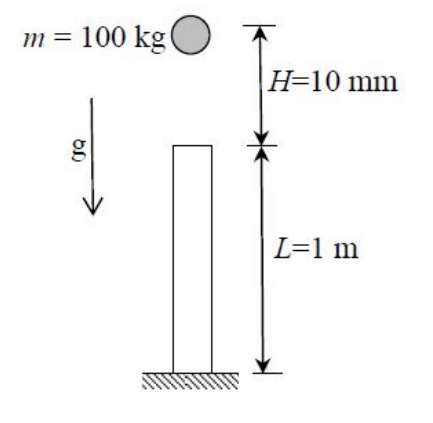
\includegraphics[width=0.5\columnwidth]{Figs/image (26).png}
    \caption*{}
    \label{fig:40}
    \end{figure} 

    \item Two disks A and B with identical mass ($m$) and radius ($R$) are initially at rest. They roll down from the top of identical inclined planes without slipping. Disk A has all of its mass concentrated at the rim, while Disk B has its mass uniformly distributed. At the bottom of the plane, the ratio of velocity of the center of disk A to the velocity of the center of disk B is:
    \hfill{\brak{\text{GATE ME 2017}}}
    \begin{enumerate}
        \begin{multicols}{4}
            \item $\sqrt{\frac{3}{4}}$
            \item $\sqrt{\frac{3}{2}}$
            \item $1$
            \item $\sqrt{2}$
        \end{multicols}
    \end{enumerate}

    \item A rectangular region in a solid is in a state of plane strain. The $(x,y)$ coordinates of the corners of the undeformed rectangle are given by $P(0,0)$, $Q(4,0)$, $R(4,3)$, $S(0,3)$. The rectangle is subjected to uniform strains, $\varepsilon_{xx} = 0.001$, $\varepsilon_{yy} = 0.002$, $\gamma_{xy} = 0.003$. The deformed length of the elongated diagonal, up to three decimal places, is $\underline{\hspace{2cm}}$ units.
    \hfill{\brak{\text{GATE ME 2017}}}

    \item A machine element has an ultimate strength ($\sigma_u$) of 600 N/mm$^2$, and endurance limit ($\sigma_{en}$) of 250 N/mm$^2$. The fatigue curve for the element on a log-log plot is shown below. If the element is to be designed for a finite life of 10000 cycles, the maximum amplitude of a completely reversed operating stress is $\underline{\hspace{2cm}}$ N/mm$^2$.
    \hfill{\brak{\text{GATE ME 2017}}}
    \begin{figure}[h]
    \centering
    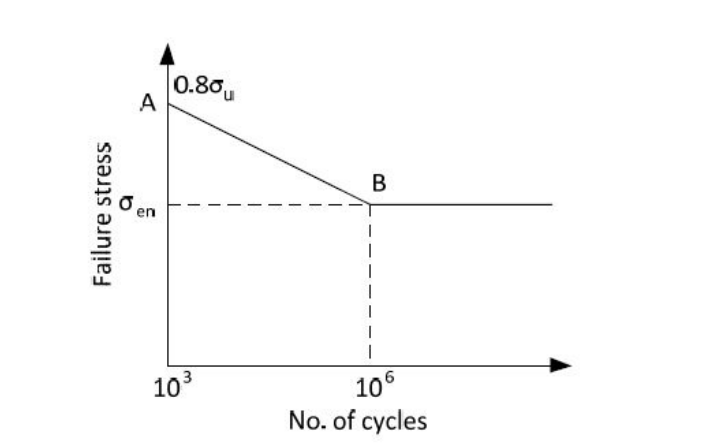
\includegraphics[width=0.5\columnwidth]{Figs/image (27).png}
    \caption*{}
    \label{fig:43}
    \end{figure}

    \item A horizontal bar, fixed at one end ($x=0$), has a length of 1 m, and cross-sectional area of 100 mm$^2$. Its elastic modulus varies along its length as given by $E(x) = 100 e^x$ GPa, where $x$ is the length coordinate (in m) along the axis of the bar. An axial tensile load of 10 kN is applied at the free end ($x=1$). The axial displacement of the free end is $\underline{\hspace{2cm}}$ mm.
    \hfill{\brak{\text{GATE ME 2017}}}

    \item In an epicyclic gear train, shown in the figure, the outer ring gear is fixed, while the sun gear rotates counterclockwise at 100 rpm. Let the number of teeth on the sun, planet and outer gears be 50, 25, and 100, respectively. The ratio of magnitudes of angular velocity of the planet gear to the angular velocity of the carrier arm is $\underline{\hspace{2cm}}$.
    \hfill{\brak{\text{GATE ME 2017}}}
    \begin{figure}[h]
    \centering
    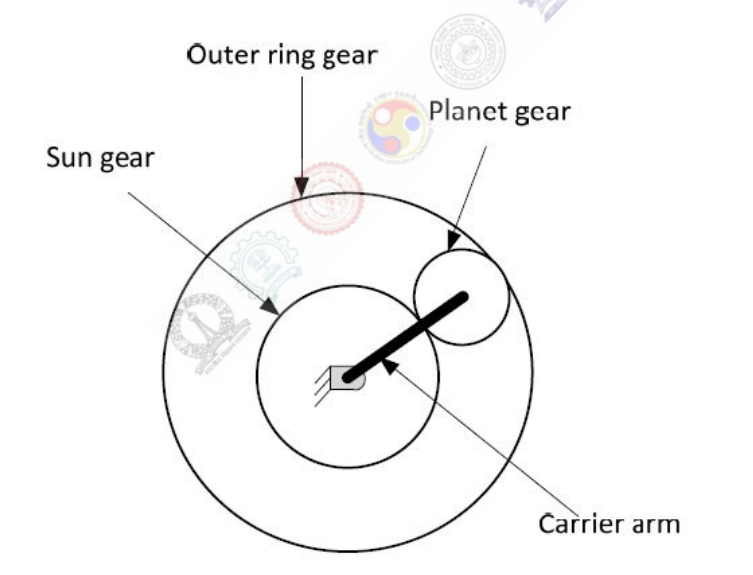
\includegraphics[width=0.5\columnwidth]{Figs/image (28).png}
    \caption*{}
    \label{fig:45}
    \end{figure}

    \item A thin uniform rigid bar of length $L$ and mass $M$ is hinged at point $O$, located at a distance of $L/3$ from one of its ends. The bar is further supported using springs, each of stiffness $k$, located at the two ends. A particle of mass $m = M/4$ is fixed at one end of the bar, as shown in the figure. For small rotations of the bar about $O$, the natural frequency of the system is:
    \hfill{\brak{\text{GATE ME 2017}}}
    \begin{figure}[h]
    \centering
    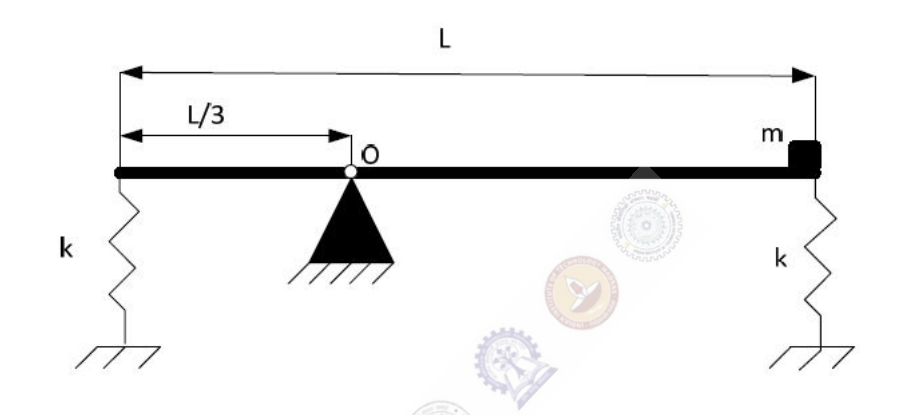
\includegraphics[width=0.5\columnwidth]{Figs/image (29).png}
    \caption*{}
    \label{fig:46}
    \end{figure}
    \begin{enumerate}
        \begin{multicols}{4}
            \item $\sqrt{\frac{5k}{M}}$
            \item $\sqrt{\frac{5k}{2M}}$
            \item $\sqrt{\frac{3k}{2M}}$
            \item $\sqrt{\frac{3k}{M}}$
        \end{multicols}
    \end{enumerate}

    \item For an inline slider-crank mechanism, the lengths of the crank and connecting rod are 3 m and 4 m, respectively. At the instant when the connecting rod is perpendicular to the crank, if the velocity of the slider is 1 m/s, the magnitude of angular velocity (up to 3 decimal points accuracy) of the crank is $\underline{\hspace{2cm}}$ radian/s.
    \hfill{\brak{\text{GATE ME 2017}}}

    \item A 10 mm deep cylindrical cup with diameter of 15 mm is drawn from a circular blank. Neglecting the variation in the sheet thickness, the diameter (up to 2 decimal points accuracy) of the blank is $\underline{\hspace{2cm}}$ mm.
    \hfill{\brak{\text{GATE ME 2017}}}

    \item Circular arc on a part profile is being machined on a vertical CNC milling machine. CNC part program using metric units with absolute dimensions is listed below:
    \hfill{\brak{\text{GATE ME 2017}}}
    \begin{verbatim}
    N60 G01 X 30 Y 55 Z -5 F50
    N70 G02 X 50 Y 35 R 20
    N80 G01 Z 5
    \end{verbatim}
    The coordinates of the centre of the circular arc are:
    \begin{enumerate}
        \begin{multicols}{4}
            \item (30, 55)
            \item (50, 55)
            \item (50, 35)
            \item (30, 35)
        \end{multicols}
    \end{enumerate}

    \item Assume that the surface roughness profile is triangular as shown schematically in the figure. If the peak to valley height is 20 $\mu$m, the central line average surface roughness $R_a$ (in $\mu$m) is:
    \hfill{\brak{\text{GATE ME 2017}}}
    \begin{figure}[h]
    \centering
    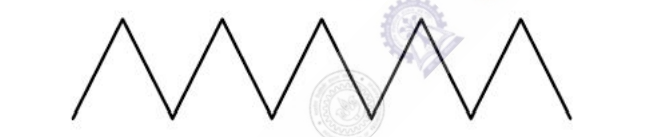
\includegraphics[width=0.5\columnwidth]{Figs/image (30).png}
    \caption*{}
    \label{fig:50}
    \end{figure}
    \begin{enumerate}
        \begin{multicols}{4}
            \item 5
            \item 6.67
            \item 10
            \item 20
        \end{multicols}
    \end{enumerate}

    \item Two models, P and Q, of a product earn profits of Rs. 100 and Rs. 80 per piece, respectively. Production times for P and Q are 5 hours and 3 hours, respectively, while the total production time available is 150 hours. For a total batch size of 40, to maximize profit, the number of units of P to be produced is $\underline{\hspace{2cm}}$.
    \hfill{\brak{\text{GATE ME 2017}}}

    \item Following data refers to the jobs (P, Q, R, S) which have arrived at a machine for scheduling. The shortest possible average flow time is $\underline{\hspace{2cm}}$ days.
    \hfill{\brak{\text{GATE ME 2017}}}

    \begin{tabular}{|c|c|}
        \hline
        Job & Processing Time (days) \\
        \hline
        P & 15 \\
        \hline
        Q & 9 \\
        \hline
        R & 22 \\
        \hline
        S & 12 \\
        \hline
    \end{tabular}

    \item A block of length 200 mm is machined by a slab milling cutter 34 mm in diameter. The depth of cut and table feed are set at 2 mm and 18 mm/minute, respectively. Considering the approach and the over travel of the cutter to be same, the minimum estimated machining time per pass is $\underline{\hspace{2cm}}$ minutes.\hfill{\brak{\text{GATE ME 2017}}}

    \item A sprue in a sand mould has a top diameter of 20 mm and height of 200 mm. The velocity of the molten metal at the entry of the sprue is 0.5 m/s. Assume acceleration due to gravity as 9.8 m/s$^2$ and neglect all losses. If the mould is well ventilated, the velocity (up to 3 decimal points accuracy) of the molten metal at the bottom of the sprue is $\underline{\hspace{2cm}}$ m/s.
    \hfill{\brak{\text{GATE ME 2017}}}

    \item Two cutting tools with tool life equations given below are being compared:
    \hfill{\brak{\text{GATE ME 2017}}}
    \begin{align*}
        \text{Tool 1: } V T^{0.1} &= 150 \\
        \text{Tool 2: } V T^{0.3} &= 300
    \end{align*}
    where $V$ is cutting speed in m/minute and $T$ is tool life in minutes. The breakeven cutting speed beyond which Tool 2 will have a higher tool life is $\underline{\hspace{2cm}}$ m/minute.

    \item He was one of my best $\_\_\_\_$ and i felt his loss $\_\_\_\_$.
    \hfill{\brak{\text{GATE ME 2017}}}
    \begin{enumerate}
        \begin{multicols}{4}
            \item friend,keenly
            \item friends,keen
            \item friend,keener
            \item friends,keenly
        \end{multicols}
    \end{enumerate}

    \item As the two speakers became increasingly agitated, the debate became $\_\_\_\_$.
    \hfill{\brak{\text{GATE ME 2017}}}
    \begin{enumerate}
        \begin{multicols}{4}
            \item lukewarm
            \item poetic
            \item forgiving
            \item heated
        \end{multicols}
    \end{enumerate}

    \item A right-angled cone (with base radius 5 cm and height 12 cm), as shown in the figure below, is rolled on the ground keeping the point P fixed until the point Q (at the base of the cone, as shown) touches the ground again.
    \hfill{\brak{\text{GATE ME 2017}}}
    \begin{figure}[h]
    \centering
    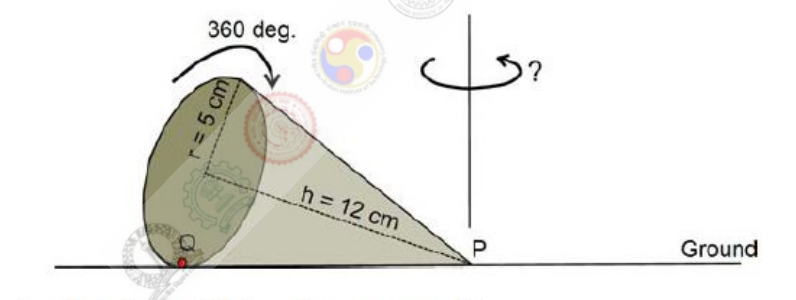
\includegraphics[width=0.5\columnwidth]{Figs/image (31).png}
    \caption*{}
    \label{fig:58}
    \end{figure}
    \newpage
    \begin{enumerate}
        \begin{multicols}{4}
            \item $\frac{5\pi}{12}$
            \item $\frac{5\pi}{24}$
            \item $\frac{24\pi}{5}$
            \item $\frac{10\pi}{13}$
        \end{multicols}
    \end{enumerate}

    \item In a company with 100 employees, 45 earn Rs. 20,000 per month, 25 earn Rs. 30,000, 20 earn Rs. 40,000, 8 earn Rs. 60,000, and 2 earn Rs. 150,000. The median of the salaries is
    \hfill{\brak{\text{GATE ME 2017}}}
    \begin{enumerate}
        \begin{multicols}{4}
            \item $Rs 20,000$
            \item $Rs 30,000$
            \item $Rs 32,300$
            \item $Rs 40,000$
        \end{multicols}
    \end{enumerate}

    \item P. Q. and R talk about S's car collection. P states that S has at least 3 cars. Q believes that S has less than 3 cars. R indicates that to his knowledge, S has at least one car. Only one of P, Q and R is right. The number of cars owned by S is
    \hfill{\brak{\text{GATE ME 2017}}}
    \begin{enumerate}
        \begin{multicols}{4}
            \item $0$
            \item $1$
            \item $3$
            \item Cannot be determined
        \end{multicols}
    \end{enumerate}

    \item "Here, throughout the early 1820s, Stuart continued to fight his losing battle to allow his sepoys to wear their caste-marks and their own choice of facial hair on parade, being again reprimanded by the commander-in-chief. His retort that 'A stronger instance than this of European prejudice with relation to this country has never come under my observations' had no effect on his superiors."
    

    According to this paragraph, which of the statements below is most accurate?
    \hfill{\brak{\text{GATE ME 2017}}}
    \begin{enumerate}
            \item Stuart's commander-in-chief was moved by this demonstration of his prejudice.
            \item The Europeans were accommodating of the sepoys' desire to wear their caste-marks.
            \item Stuart's 'losing battle' refers to his inability to succeed in enabling sepoys to wear caste-marks.
            \item The commander-in-chief was exempt from the European prejudice that dictated how the sepoys were to dress.
    \end{enumerate}

    
    
    \item What is the sum of the missing digits in the subtraction problem below?
    \hfill{\brak{\text{GATE ME 2017}}}
    \begin{figure}[h]
    \centering
    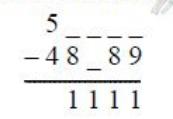
\includegraphics[width=0.2\columnwidth]{Figs/image (32).png}
    \caption*{}
    \label{fig:62}
    \end{figure}
   
    \begin{enumerate}
        \begin{multicols}{2}
            \item 8
            \item 10
            \item 11
            \item Cannot be determined
        \end{multicols}
    \end{enumerate}





  
    \item Let $S_1$ be the plane figure consisting of the points $(x, y)$ given by the inequalities $|x - 1| \leq 2$ and $|y + 2| \leq 3$. Let $S_2$ be the plane figure given by the inequalities $x - y \geq -2$, $y \geq 1$, and $x \leq 3$. Let $S$ be the union of $S_1$ and $S_2$. The area of $S$ is:
    \hfill{\brak{\text{GATE ME 2017}}}
    \begin{enumerate}
        \begin{multicols}{4}
            \item $26$
            \item $28$
            \item $32$
            \item $34$
        \end{multicols}
    \end{enumerate}



  
    \item Two very famous sportsmen Mark and Steve happened to be brothers, and played for country K. Mark teased James, an opponent from country E, ``There is no way you are good enough to play for your country.'' James replied, ``Maybe not, but at least I am the best player in my own family.''

    Which one of the following can be inferred from this conversation?
    \hfill{\brak{\text{GATE ME 2017}}}
    \begin{enumerate}
        \begin{multicols}{2}
            \item Mark was known to play better than James
            \item Steve was known to play better than Mark
            \item James and Steve were good friends
            \item James played better than Steve
        \end{multicols}
    \end{enumerate}


    \item In the graph below, the concentration of a particular pollutant in a lake is plotted over (alternate) days of a month in winter (average temperature 10 \degree C) and a month in summer (average temperature 30 \degree C).
    

     \begin{figure}[h]
    \centering
    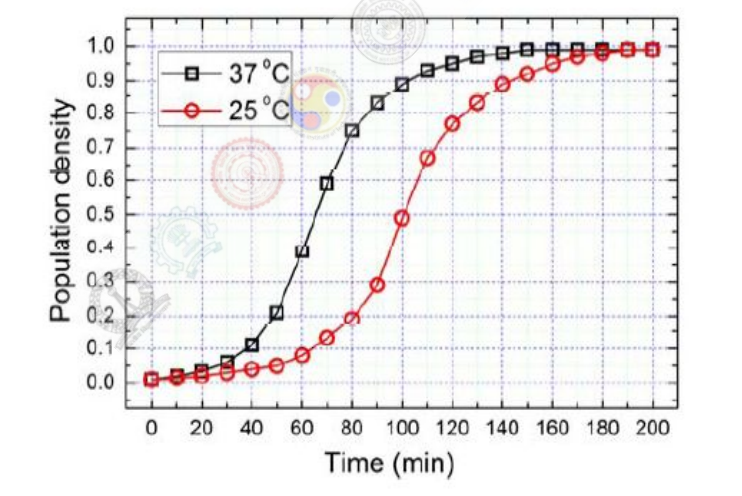
\includegraphics[width=0.5\columnwidth]{Figs/image (33).png}
    \caption*{}
    \label{fig:65}
    \end{figure}

    Consider the following statements based on the data shown above:

    i. Over the given months, the difference between the maximum and the minimum pollutant concentrations is the same in both winter and summer.

    ii. There are at least four days in the summer month such that the pollutant concentrations on those days are within 1 ppm of the pollutant concentrations on the corresponding days in the winter month.

    Which one of the following options is correct?
    \hfill{\brak{\text{GATE ME 2017}}}
    \begin{enumerate}
        \begin{multicols}{4}
            \item Only i
            \item Only ii
            \item Both i and ii
            \item Neither i nor ii
        \end{multicols}
    \end{enumerate}
\end{enumerate}
\end{document}
